\section{Dynamical models (include time)}

\subsection{Examples with one variable per time step}
% \textbf{Hidden Markov Models (HMM)}\\
% \textbf{Kalman FIlters}\\
% 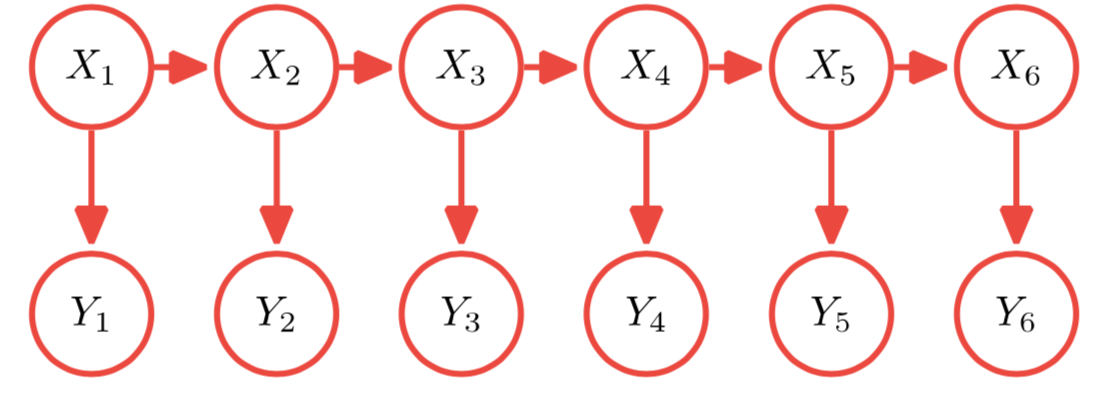
\includegraphics[scale=.25]{HMM_KF.png}\\
$X_1, ...,X_T$ (unobserved) hidden states\\
$Y_1, ...,Y_T$ (noisy) observations\\
\textbf{HMMs (polytrees: can use belief propagation):} $X_i$ categorical, $Y_i$ categorical (or arbitrary)\\
\textbf{Kalman filters:} $X_i, Y_i$ Gaussian distributions\\
- $P(X_1)$: prior belief about location at time i\\
- $P(X_{t+1}|X_t)$: \textbf{'Motion model'} (how do I expect my target to move in the environment?): 
    $X_{t+1}=FX + \epsilon_t$ where $\epsilon_t \sim N(0, \Sigma_x)$\\
- $P(Y_t|X_t)$: \textbf{'Sensor model'} (what do I observe if target is at location $X_t$?)
    $Y_t=HX_t+\eta_t$ where $\eta_t\sim N(0, \Sigma_y)$

\subsection{Inference tasks}
\textbf{Filtering}: $P(X_t|y_{1,...,t})$ Is it raining today?\\
\textbf{Prediction}: $P(X_{t+\tau}|Y_{1:t})$ Rain 5 days from now? \\
Example for one step:
$P(X_{t+1}|Y_{1:t})=\sum_x P(X_{t+1}, X_t=x_t|Y_{1:t})=\sum_x P(X_{t+1} | X_t=x_t)P(X_t|Y_{1:t})$ (with KFs, you need \textbf{integrals}!)\\
\textbf{Smoothing}: $P(X_\tau|y_{1:t})$ with $\tau<t$ Did it rain last week? [Can use sum-product (aka forward-backward).] \\
\textbf{MPE}:  $ \underset{x_{1:T}}{argmax}P(x_{1:T}|y_{1:T})$ Can use max product (aka Viterbi algorithm).\\
\textbf{Bayesian filtering:}
Start with $P(X_1)$:\\
At time t, assume we have $P(X_t|y_{1:t-1})$\\
Conditioning: 
$P(X_t|y_{1:t})= \frac{P(X_t|y_{1:t-1})P(y_t|X_t)}{\sum_{x_{t}} P(X_t|y_{1:t-1})P(y_t|X_t)}$\\
Prediction ($O(n^2)$ \textit{vs} $O(n)$ in conditioning):\\ 
$P(X_{t+1}|y_{1:t}) = \sum_x P(X_{t+1}|X_t)P(X_t|y_{1:t})$\\
\textbf{Since HMM is a polytree, smoothing/MPE can be computed by VE/BP.}
\textbf{Kalman filtering:} Bayesian filtering for continuous problems. RV corrupted by Gaussian distributions with zero mean. \textbf{Bayesian filtering is basically the same, except that sums turn to integrals.}
\textbf{General Kalman update}\\
- Transition model:
    $P(x_{t+1}|x_t)=N(x_{t+1};Fx_t, \Sigma_x)$\\
- Sensor model:
    $P(y_{t}|x_t)=N(y_{t};Hx_t, \Sigma_y)$\\
- Kalman update:\\
    $\mu_{t+1}=F\mu_t+K_{t+1}(y_{t+1}-HF\mu_t)$\\
    $\Sigma_{t+1}=(I-K_{t+1})(F\Sigma_tF^T + \Sigma_x)$\\
- Kalman gain:
    $K_{t+1}=(F\Sigma_t F^T+\Sigma_x)H^T(H(F\Sigma_t F^T+\Sigma_x)H^T+ \Sigma_y)^{-1}$


\subsection{Examples with > 1 variable per time step}
\textbf{Dynamic Bayesian Networks}: a BN at every time step\\
% 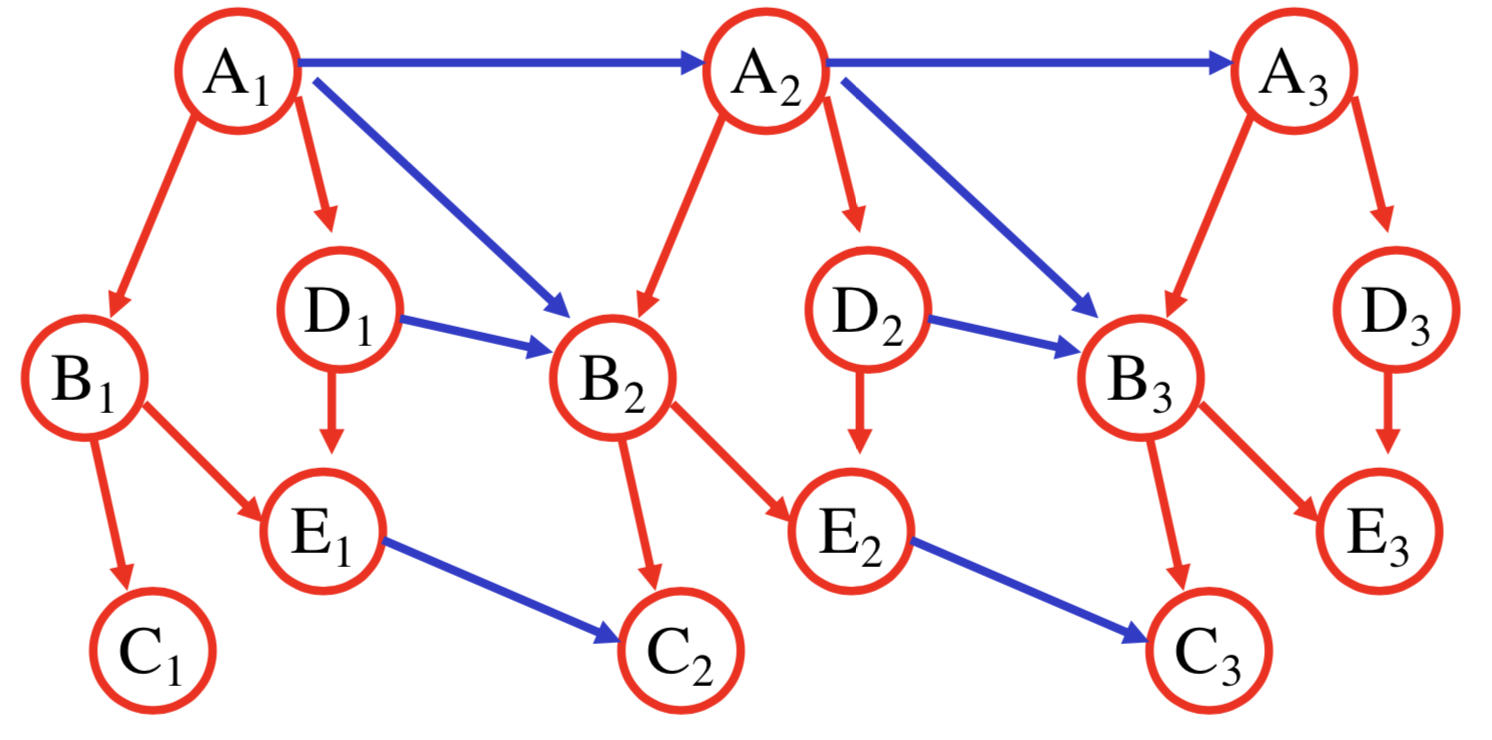
\includegraphics[scale=.1]{DBN.png}
These models typically have many loops. Exact inference is usually intractable.
\subsection{Approx. infer. for filtering (DBNs and nonlinear Kalman filters): Particle filtering}
\textbf{Suppose}: $P(X_t|y_{1:t})\approx \frac{1}{N}\sum_{i=1}^N \delta_{x_{i, t}}$, where $\delta$ is the indicator function.
\textbf{Prediction}: Propagate each particle: $x'_i \sim P(X_{t+1}|x_{i,t})$\\
\textbf{Conditioning}:\\
- weight particles $w_i=\frac{1}{Z}P(y_{t+1}|x'_i)$\\
- resample N particles $x_{i, t+1}  \sim \frac{1}{Z} \sum_{i=1}^N w_i \delta_{x'_i}$\\
% \textbf{Conclusion we came to:} $\frac{\sum_{i=1}^N w_i \delta_{x'_i}}{\sum_{i=1}^N w_i \delta_{x_i}}$
\textbf{Conclusion we came to:} $Z =\sum_{i=1}^N w_i \delta_{x_i}$
